\newpage
\section{GUI}
\label{sec:Gui}
\subsection{Bakgrunn}
GUI, graphical user interface, er et grensesnitt som lar brukerne samhandle med et dataprogram grafisk, vanligvis ved hjelp av tastatur og datamus. I motsetning til typiske shellapplikasjoner hvor man navigerer ved hjelp av kommandoer, består et grafisk grensesnitt ofte av grafiske ikoner og lydindikatorer\cite{wiki:GUI}. Grunnet den bratte læringskurven på en kommandobasert datamaskin med shellapplikasjoner ble grafisk brukergrensesnitt med mulighet for å bruke mus til å klikke på knapper, tekstfelt og informasjonsfelt raskt populært. Hos de to mest populære operativsystemene på markedet i dag, Windows og MacOS, er det GUI-et står i sentrum, mens det i UNIX er mer en blanding av et kommandobasert system og grafisk brukergrensesnitt.

Vi ønsket at det skulle være lettere å benytte våre implementasjoner diskutert i kapittel \ref{sec:Glatting} - \ref{sec:Anonymisering}, og bestemte oss for å lage vårt eget program med et grafisk brukergrensesnitt. Her skal det være mulighet for å utføre alle de implementerte operasjonene interaktivt på ulike utvalgte bilder. Vi endte opp med å bruke det foreslåtte rammeverket \texttt{PyQt5}\footnote{\url{https://pypi.org/project/PyQt5/}}, som gjør det enkelt å bruke implementasjonene vi allerede hadde skrevet med Python i GUI-applikasjonen. Ved å skrive programmet i PyQt5 kan man kjøre programmet på både Windows, MacOS og Linux, noe som forminsket arbeidsmengden betraktelig og samtidig øker portabiliteten.

\subsection{Implementasjon}
\label{sec:GUIimpl}
Programmet kjøres fra \texttt{Main.py} hvor main ligger. Vi har valgt en vindusbasert applikasjon hvor man fra hjemskjermen kan velge hvilken implementasjon man har lyst til å benytte seg av. Vi har funnet det hensiktsmessig å dele applikasjonen opp i ulike moduler, hvor det er én modul for hjemskjermen og én modul for hver av implementasjonene. Hver modul har sin egen .py-fil i mappa \texttt{src/} hvor all kode er lagret. Dette har vi gjort for å få det mer oversiktlig når vi importerer de ulike bibliotekene vi har bruk for i den aktuelle modulen.

På grunn av at vi har valgt en vindusbasert applikasjon har vi derfor laget et design for hver modul. Designet til hver modul lagres som en .ui-fil som importeres når en modul initialiseres. Designet er gjort i \texttt{Qt5 Designer}\footnote{\url{https://pypi.org/project/PyQt5Designer/}}, som gjør det enkelt å lage et oversiktlig UI med tekstfelter, knapper og bilder. Alle .ui-filene er lagret i mappa \texttt{src/}. Hver gang Main.py lastes, tilpasses applikasjonen slik at den oppfører seg likt på skjermer med ulik pikseltetthet.

\begin{lstlisting}[language=Python]
QtWidgets.QApplication.setAttribute(QtCore.Qt.AA_EnableHighDpiScaling,True)
QtWidgets.QApplication.setAttribute(QtCore.Qt.AA_UseHighDpiPixmaps,True)
\end{lstlisting}

Når en modul initialiseres må vinduets dimensjoner justeres. Dette må gjøres fordi designet er laget med Qt5 Designer, og oppfører seg derfor annerledes på skjermer med ulike dimensjoner. Disse justeringene gjøres ved hjelp av funksjonen adjustScreen(). Her får man dimensjonen ved å hente skjermens høyde og bredde, og bruker denne til å justere vinduet. Hvert vindu er forskjellig fra hverandre, og derfor har hver modul sin egen adjustScreen() funksjon.

\begin{lstlisting}[language=Python]
def adjustScreen(self):
    screenWidth = app.primaryScreen().size().width()
    screenHeight = app.primaryScreen().size().height()
    if screenWidth/screenHeigh == 1.5:
        width = int(screenWidth / 1.8)
        height = int(screenHeight / 2)
    else:
        width = int(screenWidth / 2.22222)
        height = int(screenHeight / 1.95298)
    self.setGeometry(500, 80, width, height)
\end{lstlisting}
\newpage
Hjemskjermen består av et antall knapper med tilhørende tekst som forklarer hva den aktuelle implementasjonen gjør. Når man klikker på en knapp opprettes en dialog til denne modulen. Hvis det lykkes med å opprette en dialog vil et nytt vindu åpnes hvor den aktuelle modulens design og funksjonaliteter vises. 

Hovedelementet i hver modul er bildet som vises i bilderammen, se figurene \ref{fig:guiexample}, \ref{fig:guiexample2} og \ref{fig:guiexample3}. Vi har valgt å bruke MatPlotLib til å vise bilder, noe som gjør at vi kan bruke \texttt{plt.imshow()}\footnote{\url{https://matplotlib.org/3.2.1/api/_as_gen/matplotlib.pyplot.imshow.html}} som vi har brukt i hver enkelt implementasjon i Jupyter Notebook-filene. I vår applikasjon er dette en bedre metode å vise bilder på sammenliknet med alternativet hvor vi da ville brukt QLabel og \texttt{setPixMap}\footnote{\url{https://doc.qt.io/archives/qt-4.8/qlabel.html\#pixmap-prop}}. Selve bildet er en imagewidget av typen FigureCanvas, og vi har derfor opprettet en egen klasse \texttt {imagewidget} i filen \texttt{src/imagewidget.py}. Ved oppstart av hver modul initialiseres imagewidget hvor \texttt{self.img} opprettes og initialiseres. Hver gang et nytt bilde skal vises kalles \texttt{showImage(self, image, colour=True)}. Her blir det lagt til subplot, aksene fjernes og bildet justeres slik at det fyller mest mulig av bilderammen. Avhengig av om colour er True eller False, vises enten et fargebilde eller et gråtonebilde ved bruk av imshow(). Det er i hver modul lagret \texttt{self.path} som hele tiden er oppdatert med filstien til bildet som er valgt. Denne benyttes når brukeren vil se et annet bilde eller fjerne effekten gjort på bildet og vise originalbildet. Sett bort fra \texttt{Anonymisering.py} har hver modul har også en lokal variabel \texttt{self.image} hvor det bildet som vises i applikasjonen ligger lagret som en numpy array. Denne sendes til \texttt{FunctionGUI/saveImage} når brukeren vil lagre bildet. Her åpnes en \texttt{QFileDialog}\footnote{\url{https://doc.qt.io/qt-5/qfiledialog.html}}, som returnerer ønsket navn på filen og filsti til ønsket mappe.

I hver modul importeres klassen \texttt{showCode(QMainWindow)} fra \texttt{FunctionGUI.py} som viser koden i et nytt vindu for implementasjonen. Koden som vises ligger lagret i en .txt-fil i \texttt{src/codes}, som vises ved å bruke funksjonen \texttt{FunctionGUI/ShowCode}. Her opprettes det et nytt \texttt{QMainWindow}, hvor koden vises i et rullbart tekstfelt. 
\\[1cm]
\begin{figure}[H]
\begin{center}
    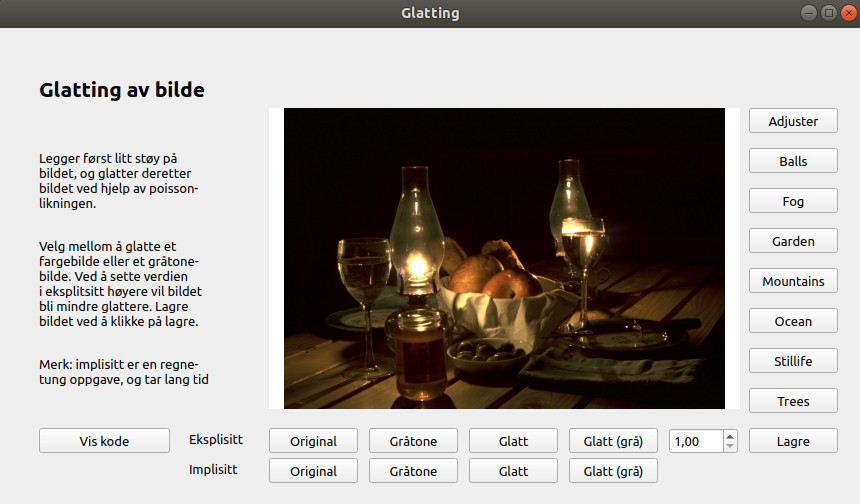
\includegraphics[width=0.9\columnwidth]{bilder/Gui/guiexample.jpg}
     \caption{Grafisk brukergrensesnitt - Glatting (Linux) \label{fig:guiexample}}
\end{center}
\end{figure}
\newpage
\subsubsection{Glatting}
Et bilde kan glattes ved å bruke en eksplisitt løsning av diffusjonslikningen. Dette gjøres av funksjonen \texttt{blurImage(self, colour)}. Denne henter først et fargebilde hvis colour er True eller gråtonebilde hvis colour er False. Videre lages en kopi av originalbildet som det legges litt støy på, før dette glattes ved å bruke funksjonen \texttt{eksplisittGlatting()} fra \texttt{Eksplisitt.py}. Tilslutt vises bildet ved å bruke modulens showImage-funksjon.

Bildet kan også glattes ved å bruke en implisitt løsning av diffusjonslikningen. Dette gjøres av funksjonen \texttt{blurImageImplsitt(self, colour=True)}. Hvis colour er True leses det inn et fargebilde, og hvis colour er False leses det inn et gråtonebilde ved bruk av \texttt{grayscale()} fra \texttt{Grayscale.py}. Disse bildene lagres som en numpyarray \texttt{u} som videre omformes til å inneholde verdier mellom 0 og 1, hvor verdier over 1 og under 0 klippes til lovlige verdier. Deretter glattes bildet \texttt{u} ved å bruke funksjonen \texttt{implisitt()} fra \texttt{implisitt.py}. Tilslutt vises bildet ved å bruke showImage-funksjonen i modulen.

\subsubsection{Inpainting}
I Inpainting sitt GUI kan man få vist bildet med manglende informasjon før det fylles inn. Dette gjøres ved å bruke funksjonen \texttt{showMask(self, number)}, som bruker med \texttt{self.getPath} og \texttt{self.number} til å finne filstien til bildet. Denne filstien sendes med til funksjonen \texttt{maskImage()} fra \texttt{Inpainting.py} som returnerer bildet med masken. Informasjonen i bildet fylles inn i funksjonen \texttt{inpaint(self, number)}, som sender bruker \texttt{self.getPath} og \texttt{self.number} til å finne filstien til bildet. Dette sendes til \texttt{Inpaint()} fra \texttt{Inpainting.py} som returnerer et bilde hvor informasjonen er fylt inn, som vises av \texttt{showImage()}. 

\subsubsection{Kontrastforsterkning}
Når knappen \texttt{contrastColour} trigges starter funksjonen \texttt{contrastImage(self)}. Denne funksjonen kaller på \texttt{contrastEnhance()} fra \texttt{contrastEnhancement.py} og sender med \texttt{self.path} og den aktuelle verdien på \texttt{QDoubleSpinBox}\footnote{\url{https://doc.qt.io/qtforpython/PySide2/QtWidgets/QDoubleSpinBox.html}} som brukeren har satt en verdi på. \newline\texttt{contrastEnhancement()} returnerer et kontrastforsterket bilde som vises i GUI av \newline\texttt{showContrastImage(self, im, colour=True)}. Hvis brukeren trigger knappen \texttt{contrastOrigGray} startes funksjonen \texttt{contrastGrayImage(self)}. Her sendes \texttt{self.path} og verdien på \newline\texttt{QDoubleSpinBox} med til \texttt{contrastEnhanceBW()} i \texttt{contrastEnhancement.py}, og returnerer et kontrastforsterket gråtonebilde. Dette vises av \texttt{showContrastImage()}.

\subsubsection{Demosaicing}
Det er mulig å bruke to forskjellige metoder for å gjøre demosaicing på et bilde i denne modulen. Hvis man vil bruke metoden som innebærer at man manuelt fyller inn informasjonen fra gråtonemosaikken inn i hver fargekanal, oppretter en maske for fargekanalene og inpainter den manglende informasjonen med bruk av diffusjonslikningen, kan dette gjøres med \texttt{demosaicImage()}. Denne bruker \texttt{mosaicToRGB()} til å utføre demosaicingen, som vises på skjermen ved å bruke \texttt{showImage()}. Hvis man har lyst til å se gråtonemosaikken før informasjonen inpaintes gjøres dette av \texttt{mosaic()}, hvor gråtonemosaikken returneres av \texttt{getMosaic()} og vises av \texttt{showImage()}. Ønsker man heller bruke biblioteket \texttt{Colour-demosaicing}\footnote{\url{https://pypi.org/project/colour-demosaicing/}} til å gjøre demosaicing av bildet gjøres dette ved å bruke \texttt{demosaicImagePackage}. Her brukes først \texttt{Colour} til å lage en gråtonemosaikk, før denne gråtonemosaikken demosaices ved å bruke \texttt{Colour-demosaicing}. Hvis man har lyst til å se gråtonemosaikken som lages med dette biblioteket gjøres dette med \texttt{mosaicPackage()}. Gråtonemosaikken og demosaicbildet vises begge med \texttt{showImage()}.

\subsubsection{Sømløs kloning}
For å sømløst klone en av de tre forhåndsvalgte sammensetningene av bilder brukes \newline\texttt{seamlessImage(self, number, img1, img2)}.
\texttt{Self.number} er en integer som holder verdien på hvilken av kombinasjonene som klones. Deretter sjekkes verdi på den aktuelle av de tre lokale boolvariablene. Disse boolvariable fungerer som status på om noen av de tre forhåndsvalgte kombinasjonene av bilder allerede er regnet ut. Disse settes til False ved oppstart av modulen, og oppdateres til True hvis den aktuelle kombinasjonen av bilder er blitt klonet. Dette er gjort fordi det å sømløst klone et bilde er en regnetung oppgave og tar lang tid, og ved å lagre bildet kan brukeren raskt kan sammenlikne bildet før og etter kloning. Før det sjekkes om den aktuelle boolverdien er False, settes bildet i bilderammen til originalversjonen av bildet som det skal klones inn i. Dette er gjort for å hindre at man skal få en feilmelding om i forbindelse med bildets shape. Er boolverdien False sendes informasjon om hvor bildet skal klones, hvilket del av bildet og hvor stort dette området er med til \texttt{seamless(img1, img2, xy0, xy1, xlen, ylen)}. Deretter lagres bildet i dens aktuelle \texttt{self.imageX}, hvor X er self.number, før den aktuelle \texttt{self.imgXReady} settes til True. Er boolverdien True er dette allerede gjort og \texttt{showImage()} kan vise det ferdig klonede bildet. 

\subsubsection{Konvertering av fargetone til gråtone}
Når den enkle metoden for å konvertere et bilde til gråtone skal benyttes, brukes \texttt{convertGrayEasy()} til å kalle på funksjonen \texttt{grayscale}. Her returneres gråtonebildet som sendes til \texttt{showImage()} som viser bildet på skjermen. Velges den mer sofistikerte metoden for å konvertere et gråtonebilde brukes \texttt{convertGrayAdvanced()}. Her returneres det et gråtonebilde fra \texttt{rgb2gray()} som vises på skjermen av \texttt{showImage()}.

\begin{figure}[H]
\begin{center}
    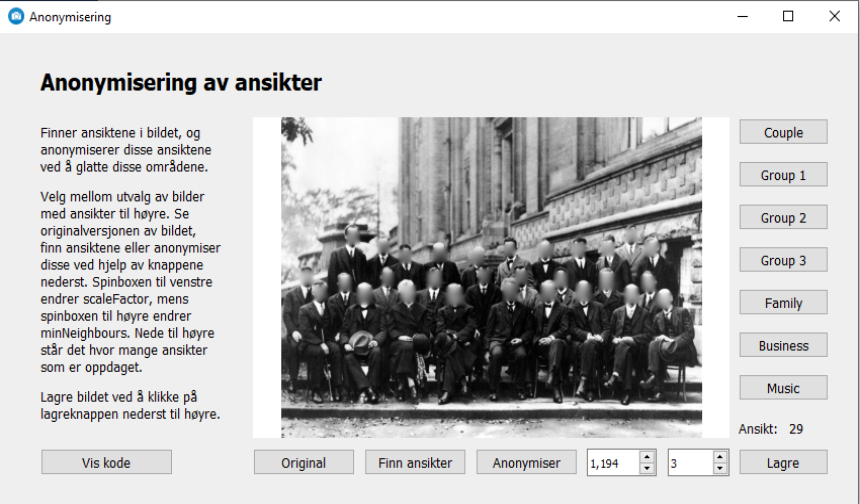
\includegraphics[width=0.9\columnwidth]{bilder/Gui/guiExampleAnon.png}
     \caption{Grafisk brukergrensesnitt - Anonymisering (Windows) \label{fig:guiexample2}}
\end{center}
\end{figure}

\subsubsection{Anonymisering}
Når GUI-et til Anonymisering lastes, blir hvert bilde nummerert og hvert bilde blir lastet inn i en variabel. Dette er gjort med hensyn til funksjonalitet for å kunne lagre bilde, og en felles bildevariabel slik som det er gjort i de andre modulene gjorde det vanskelig grunnet bruk av cv2 til å oppdage ansikt og anonymisere disse. Hver gang et nytt bilde velges hentes det aktuelle bildes filsti ved bruk av \texttt{getPath(self, nr)} og bildet leses inn og vises av \texttt{showImage()}. Variabelen \texttt{self.number}, som sier hvilket bilde som vises, blir også oppdatert, mens \texttt{self.updateCount(self, count)} oppdaterer variabelen \texttt{self.faceCount} som sier hvor mange ansikt som er blitt oppdaget. \texttt{detectFaces(file, scaleFactor, minNeighbours)} brukes til å finne ansikt på et bilde, hvor \texttt{self.getPath(self.number))} brukes til å finne filsti som sendes med som \texttt{file}. Fra \texttt{detectFaces()} returneres antallet ansikter på bildet og et bilde hvor ansiktene er markerte. Bildet vises ved å bruke \texttt{showFaces()}. For å anonymisere ansiktene brukes \texttt{anonymiseFaces()} som selv bruker \texttt{blurFace(file, scaleFactor, minNeighbours)} til å returnere antall ansikter som er oppdaget og et bilde med de anonymiserte ansiktene. Deretter oppdateres \texttt{self.number} til antall ansikter som er oppdaget, før bildet vises av \texttt{showImage()}.

\subsection{Brukermanual}
Applikasjonen startes ved å kjøre \texttt{Main.py} fra \texttt{src/} med en Pythonkompilator som støtter Python3 eller nyere, eller ved å kjøre \texttt{Main.py} med Python3 fra terminalen. Følgende biblioteker er nødvendig å ha installert for å kjøre applikasjonen:
\begin{itemize}[noitemsep,topsep=0pt,parsep=0pt,partopsep=0pt]
  \item[-] PyQt5
  \item[-] MatPlotLib
  \item[-] Numpy
  \item[-] Imageio
  \item[-] Colour
  \item[-] Colour-Demosaicing
  \item[-] cv2
\end{itemize}
Disse bibliotekene kan enkelt installeres ved å kjøre følgende kommandoer fra \texttt{imt3881-2020-prosjekt/}:
\begin{lstlisting}[language=Bash]
pip install -r requirements.txt
cd src
python Main.py
\end{lstlisting}
Når applikasjonen starter er det første som vises et vindu som viser oversikt over alle implementasjonene og hva de gjør. For å benytte seg av en implementasjon trykker man på en knappene til venstre for teksten, og et nytt vindu med den aktuelle implementasjonen vil åpnes. Nederst på startvinduet finner man knappen \texttt{Om oss}, som åpner et nytt vindu når den trigges. Det nye vinduet viser en tekst med informasjon om gruppen og emnet, i tillegg til en morsom animasjonen nederst i vinduet.
\begin{figure}[H]
\begin{center}
    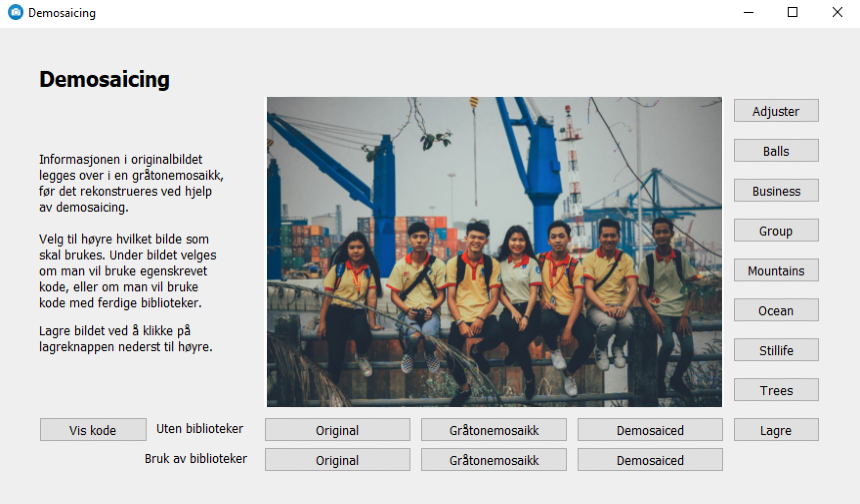
\includegraphics[width=0.9\columnwidth]{bilder/Gui/DemosaicingGuiExample.png}
     \caption{Grafisk brukergrensesnitt - Demosaicing (Windows) \label{fig:guiexample3}}
\end{center}
\end{figure}

\newpage

\subsubsection{Glatting}
Når et nytt vindu med Glatting av bilde åpnes vil et standardbilde være lastet inn. Til venstre er det informasjonstekst om hva implementasjonen gjør, en liten instruksjon på hvordan det brukes og merknad om glatting av bilde med implisitt løsning. Nede til venstre under informasjonsteksten er det en "Vis Kode"-knapp som åpner et nytt vindu hvor koden som står bak implementasjonen vises i et scrollbart tekstfelt. Under bildet er det to rader med 4 knapper hvor den øverste raden med knapper glatter bildet med en eksplisitt løsning, og den nedereste raden glatter bildet implisitt løsning. Velger man eksplisitt løsning har man også mulighet til å stille inn en verdi i spinboxen til høyre mellom 1 og 5, hvor bildet glattes mest når verdien er 1 og minst når verdien er 5. Til høyre for bildet er det åtte knapper, som gjør at brukeren kan velge mellom åtte forhåndsvalgte bilder og dermed endre hvilket bildet som skal glattes. Nede til høyre under disse knappene er det en "Lagre"-knapp som gir brukeren mulighet til å lagre bildet i .png-format eller .jpg-format lokalt på PC-en. 

\subsubsection{Inpainting}
Ved åpning av nytt vindu med Inpainting er det lastet inn et standardbilde. Til venstre er det mulig å velge mellom tre valgte eksempelbilder. Ved å klikke på knappen \texttt{maske} under den valgte eksempelknappen vises bildet med masken over. For å inpainte den manglende informasjonen i bildet klikker man på knappen \texttt{Inpaint}, og det inpaintede bildet vil etterhvert vises i bildefeltet. Til venstre for bildet er det en informasjonstekst som sier hva implementasjonen gjør og kort om hvordan man benytter seg av den. Nederst til venstre er det to knapper hvor \texttt{Vis Kode} viser koden bak implementasjonen, mens \texttt{Lagre} gir brukeren mulighet til å lagre bildet i .png-format eller .jpg-format lokalt på PC-en.

\subsubsection{Kontrastforsterkning}
Det er lastet inn et standardbilde i bilderammen når et nytt vindu med kontrastforsterkning åpnes. Dette bildet kan endres ved å klikke på en av de 8 øverste knappene til høyre. Under disse knappene er det en knapp \texttt{Lagre} som gir brukeren mulighet til å lagre det kontrastforsterkede bildet lokalt på PC-en i .png-format eller .jpg-format. Under bilderammet er det fire knapper og en spinbox. Her har brukeren mulighet til å se originalbildet, en gråtoneversjon av bildet, kontrastforsterke bildet i farger eller kontrastforsterke bildet i gråtoner. Verdien i spinboxen går fra 1 til 3, og ved å sette verdien høyere vil kontrasten økes mer. Til venstre for bildet er det en informasjonstekst som forteller hva implementasjonen gjør og kort om hvordan man bruker applikasjonen. Nederst til venstre er det en knapp \texttt{Vis Kode} som åpner et nytt vindu hvor implementasjonens kode vises.
\subsubsection{Demosaicing}
Når et nytt vindu med demosaicing åpnes vil et standardbilde være lastet inn. Dette bildet kan endres ved å klikke én av åtte øverste knappene til høyre for bildet, hvor hver knapp representerer hvert sitt bilde. Til venstre for bildet er det en informasjonstekst som forteller kort hva implementasjonen gjør og hvordan man kan bruke den. Under bildet kan man velge to måter å gjøre demosaicing av bildet på. De tre knappene på den øverste raden bruker våre egenlagde funksjoner, mens de tre knappene på den nederste raden bruker biblioteker fra Colour som nevnt i seksjon \ref{sec:GUIimpl}. Klikker på \texttt{Gråtonemosaikk} vises gråtonemosaikken av bildet med den valgte metoden. For å demosaice bilde klikker man på \texttt{Demosaiced} og bildet vises i bilderammen. Nederst til venstre er det en knapp \texttt{Vis Kode} som åpner et nytt vindu hvor koden som brukes for å demosaice et bilde vises i et scrollbart tekstfelt. Nederst til høyre finner man knappen \texttt{Lagre} som gir brukeren mulighet til et .png-bilde eller et .jpg-bilde lokalt på PC-en.

\subsubsection{Sømløs kloning}
Ved åpning av et nytt "sømløs kloning"-vindu er det lastet inn et standardbilde. Til høyre er det knapper som representerer de tre kombinasjonene av bilder som kan sys sammen. Ved å klikke på \texttt{bilde 1} eller \texttt{bilde 2} vises originalversjonen av det bildet, og man syr sammen disse to bildene ved å klikke på \texttt{Sy sammen}. Til venstre for bildet er det en informasjonstekst som forteller kort om hva implementasjonen gjør og hvordan man bruker den. Nede til venstre er det to knapper. \texttt{Vis Kode} åpner et nytt vindu med et scrollbart tekstfelt som viser brukeren koden bak implementasjonen, mens \texttt{Lagre} gir brukeren mulighet til å lagre bildet lokalt på datamaskinen.

\subsubsection{Konvertering av fargetone til gråtone}
Når brukeren åpner et nytt vindu med Konvertering til gråtone er det alltid lastet inn et standardbilde. Til venstre for dette bildet er det en informasjonstekst som forteller kort om hva implementasjonen gjør og forklarer hvordan man bruker den. Under bildet er det tre knapper som henholdsvis viser originalversjonen av bildet, viser et gråtonebilde hvor den enkle versjonen av konvertering er brukt og viser et gråtonebilde hvor den avanserte løsningen er brukt. Til høyre for bilde er mulig å velge mellom åtte forskjellige bilder, mens det nede til høyre er en lagreknapp som gir brukene mulighet til å lagre gråtonebildet. Nederst til venstre finner man knappen \texttt{Vis Kode} som åpner et nytt vindu hvor koden bak implementasjonen vises for brukeren.


\subsubsection{Anonymisering}
Når et nytt vindu med anonymisering av ansikter åpnes er det lastet inn et standardbilde i bilderammen. Dette bildet kan endres ved å klikke på én av de åtte knappene til høyre for bildet. For å vise originalversjonen av bildet hvor ingen ansikter er funnet klikker man på \texttt{Original}. Ønsker man å finne ansiktene på bildet uten å anonymisere dem klikker man på \texttt{Finn ansikter}. For å anonymisere ansiktene klikker man på \texttt{Anonymiser}, og et bilde med anonymiserte ansikter vises i bilderammen. Når brukeren enten har klikket på \texttt{Finn ansikter} eller \texttt{Anonymiser} oppdateres teksten nede til høyre for bildet med hvor mange ansikter som er funnet på bildet. De to spinboxene til høyre under bildet gir mulighet for å finpusse ansiktsgjenkjenningen. Spinboxen til venstre endrer scaleFactor for bildet og spinboxen til høyre endrer minNeighbours. Disse verdiene er satt på forhånd slik at det ansiktene i bildet skal markeres, og bør ikke endres på hvis man ikke vil ha uanonymiserte ansikter. Nederst til høyre er det en lagreknapp som gir brukeren mulighet til å lagre et bilde med anonymiserte eller markerte ansikter i .png-format eller .jpg-format. Nederst til venstre finner man knappen \texttt{Vis Kode} som viser koden bak implementasjonen i et nytt vindu. 

